In this chapter we move away from the ScatterNet ideas from the previous 
chapters and instead look at using the wavelet domain as a new space in which to
learn. In particular the ScatterNet, and even the learnable ScatterNet proposed
in the previous chapter, are built around taking complex magnitudes of the
highpass wavelets. This inherently builds invariance to shifts but at the cost
of making things smoother. In many ways this was beneficial, as it allowed us to
subsample the output and we saw that the scattering layers worked well just 
before downsampling stages of a CNN\@. However, we would now like to explore
if it is possible and at all beneficial to learn with wavelets without taking
the complex magnitude. This means that the frequency support of our activations
will remain in the same space in the Fourier domain. 

The inspiration to this chapter is the hope that learning in the
frequency/wavelet domain may afford simpler filters than learning in the pixel
domain. A classic example of this is the first layer filters in AlexNet shown in
\autoref{fig:ch6:alexnet}. These could be parameterized with only a few nonzero
wavelet coefficients, or alternatively, we could take a 
decomposition of each input channel and keep individual
subbands (or equivalently, attenuate other bands), then take the inverse wavelet
transform. 

\begin{figure}[bt]
  \centering
  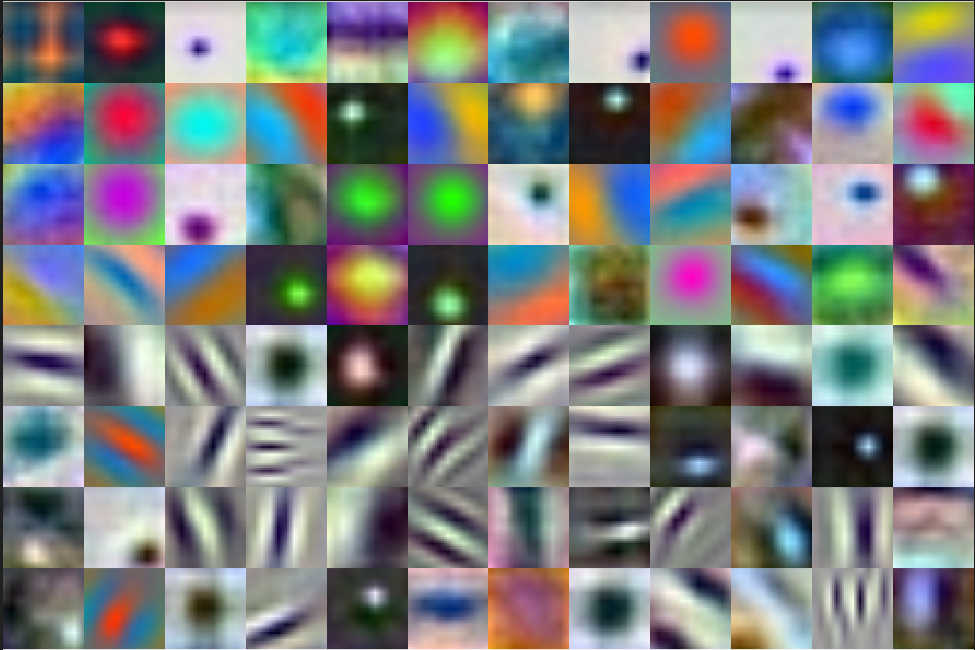
\includegraphics[width=0.7\textwidth]{\imgpath/alexfilters.png}
  \mycaption{First layer filters of the AlexNet architecture}{The first layer
  filters of the seminal AlexNet \cite{krizhevsky_imagenet_2012} are an
  inspiration for considering learning filters in the wavelet domain. Each of
  these $11\x 11$ filters would only require a handful of non zero coefficients
  in the wavelet domain. The weights shown here were taken from a pretrained
  network from torchvision \cite{marcel_torchvision_2010}.}
  \label{fig:ch6:alexnet}
\end{figure}

Our experiments show that \ldots \textbf{FINISH ME}


\section{A Summary of Choices}
As mentioned in the inspiration for this chapter, many filters that
have complex support in the pixel domain would have simple support in the
wavelet domain, but as the previous section showed, naively reparameterizing
things in a different domain may not afford us any benefit in the optimization
procedure.

There are two possible ways we can try to leverage the wavelet domain for
learning: 

\begin{enumerate}
  \item We can reparameterize filters in the wavelet domain if we use nonlinear
  optimizers like ADAM, or $\ell_1$ regularization to impose sparsity. This is
  presented in \autoref{sec:ch6:reparameterization}.
  \item We can take wavelet transforms of the inputs and learn filters on the
    wavelet coefficients. We can also apply nonlinearities to the wavelet coefficients
    such as wavelet shrinkage. On the output of this, we have the choice of either
    staying in the wavelet domain or returning to the pixel domain with an
    inverse wavelet transform. This is presented in \autoref{sec:ch6:gainlayer}
\end{enumerate}

This chapter explores both possible methods and the merits and drawbacks of
each.
